\chapter{Der Money-Coutts-Prozess}

Der Money-Coutts-Prozess beschreibt die iterative Erzeugung von Kreisen in einem Polygon.
Gegeben sind dabei ein Polygon $P$ und ein Kreis $C_1$, der zwei Seiten des Polygons berührt.
Diese Seiten berühren sich in der Ecke $A_1$ des Polygons $P$.
Weiterhin sei festgelegt, ob die folgenden Kreise gegen oder mit dem Uhrzeigersinn in der jeweils nächste Ecke des Polygons positioniert werden.
Der neue Kreis $C_2$ soll so positioniert werden, dass er den Kreis $C_1$ berührt.

Das Zentrum eines solchen Kreises liegt dabei immer auf der Winkelhalbierenden des Winkels der Ecke, in die der Kreis positioniert wird.
Kennt man den Radius des zu positionierenden Kreises, so ist die Position des Zentrums eindeutig.
Intuitiv schiebt man das Zentrum des Kreises entlang der Winkelhalbierenden so nah an die Ecke des des Polygons,
dass der Kreis die beiden anliegenden Seiten der Ecke berührt.

\citet{Taba2013} merken dazu an,
% TODO: Anmerkungen zum MCP: kleinerer Kreis wählen, preconditions

In dieser Arbeit werden folgende Konventionen zur Notation verwendet,:
Im gegebenen Polygon $P$ mit Ecken $A_1$ bis $A_n$ sind sei die Seite $a_i$ zwischen den Ecken $A_i$ und $A_{i+1}$.
Die Größe des Winkels in der Ecke bei $A_i$ beträgt $2\alpha_i$.
Das Winkelmaß $\alpha_i$ ist also gerade die Hälfte des Winkels bei $A_i$.

\begin{figure}[htbp]
    \begin{tikzpicture}
    \draw
    (3,0) coordinate (a) node[right] {a}
    -- (0,0) coordinate (b) node[left] {$A_1$}
    -- (2,2) coordinate (c) node[above right] {c};
    % \draw pic["$\alpha_1$", draw=orange, <->, angle eccentricity=1.2, angle radius=1cm]{angle=a--b--c};

\end{tikzpicture}
    \caption{Darstellung der Notationen}
\end{figure}

Um die

\begin{figure}[htbp]
    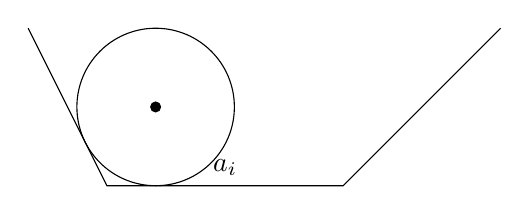
\begin{tikzpicture}
    % TODO: finish this
    \draw (0,2) -- (1,0) coordinate (a)
    -- (4,0) coordinate (b)
    -- (6,2);
    \draw (2.5,0) node[anchor=south] {$a_i$};
    % is this the golden ratio?
    \draw (1.618,1) circle (1cm);
    \fill (1.618,1) circle (2pt);
\end{tikzpicture}
    \caption{Zwei aufeinander folgende Kreise im Money-Coutts-Prozess.}
\end{figure}


